\documentclass[preprint,12pt]{elsarticle}

\usepackage{amsmath,amssymb}
\usepackage{graphicx}
\usepackage{booktabs}
\usepackage{tabularx}
\usepackage{microtype}
\usepackage{hyperref}
\pdfstringdefDisableCommands{\def\corref#1{}\def\fnref#1{}}
\usepackage{lineno}

\setlength{\emergencystretch}{2em}

\journal{Informatics in Medicine Unlocked}

\begin{document}

\begin{frontmatter}

\title{ClinicalAlign-AD: A Reproducible Multimodal Evaluation of Clinical, Plasma NfL, DTI, and Structural MRI Features for MCI-to-Alzheimer's Disease Conversion Prediction}

\author[inst1]{Jina Babanzadeh}
\ead{Jinababanzadeh@gmail.com}
\author[inst2]{Makan H.S. Javadi}
\ead{makan.hsjavadi.00@sharif.edu}
\author[inst3]{Elham Gholami Mateki}
\ead{elham.gholami.mtk@gmail.com}
\author[inst4]{M.K.Dadsetani\corref{cor1}\fnref{orcid1}}
\ead{m.dadsetani@shahed.ac.ir}
\cortext[cor1]{Corresponding author.}
\fntext[orcid1]{ORCID: \url{https://orcid.org/0009-0002-9540-7593}}

\affiliation[inst1]{
    organization={Bone, Joint and Related Tissue Research Center, Akhtar Orthopedic Hospital, Shahid Beheshti University of Medical Sciences},
    city={Tehran},
    country={Iran}
}

\affiliation[inst2]{
    organization={Department of Computer Engineering, Sharif University of Technology},
    city={Tehran},
    country={Iran}
}

\affiliation[inst3]{
    organization={Independent Researcher},
    city={Tehran},
    country={Iran}
}

\affiliation[inst4]{
    organization={Department of Computer Engineering, Faculty of Engineering, Shahed University},
    city={Tehran},
    country={Iran}
}

\begin{abstract}

\textbf{Background:}
Prediction of progression from mild cognitive impairment (MCI) to Alzheimer's disease (AD) is complicated by incomplete biomarker and imaging availability and by limited reproducibility of cohort and preprocessing decisions. This study presents a transparent, leakage-controlled evaluation of multimodal ADNI-derived data for 36-month conversion prediction.

\textbf{Methods:}
Longitudinal diagnosis records were harmonized using an explicit cohort rule. The resulting candidate cohort included 702 participants with baseline MCI, comprising 255 converters and 447 stable participants. Baseline clinical characteristics, plasma neurofilament light chain (NfL), diffusion tensor imaging (DTI), and FreeSurfer-derived structural MRI features were matched using predefined temporal windows and modality-specific quality control. A participant-disjoint stratified split contained 561 training and 141 held-out test participants. L2-regularized logistic regression, Gaussian naive Bayes, and k-nearest-neighbor models were tuned using training-only cross-validation. Confidence intervals were estimated using 1,000 class-stratified bootstrap samples.

\textbf{Results:}
Clinical variables were nearly complete, whereas NfL and primary DTI features were available for 336 (47.9\%) and 127 (18.1\%) participants, respectively. In prespecified logistic-regression ablations, clinical core features achieved an AUC of 0.580 (95\% CI 0.486--0.674), clinical extended features plus NfL achieved 0.678 (0.590--0.762), and clinical extended features plus DTI achieved 0.636 (0.547--0.727). Exploratory structural MRI analysis achieved an AUC of 0.780 (0.703--0.848), while the exploratory all-modality configuration achieved 0.802 (0.730--0.872). Complete-case DTI evaluation was infeasible because the test subset contained only four converters.

\textbf{Conclusions:}
NfL provided a modest improvement over clinical characteristics, while sparse DTI availability limited reliable complete-case evaluation. Structural MRI findings were stronger but remain exploratory and require independent validation. Explicit cohort rules, temporal matching, training-only preprocessing, and uncertainty reporting were essential for distinguishing reproducible findings from results driven by limited or informative modality availability.

\end{abstract}

\begin{keyword}
Alzheimer's disease \sep mild cognitive impairment \sep ADNI \sep neurofilament light chain \sep diffusion tensor imaging \sep FreeSurfer \sep missing modalities \sep reproducible machine learning
\end{keyword}

\end{frontmatter}

\linenumbers

\section{Introduction}

Alzheimer's disease (AD) is a progressive neurodegenerative disorder and a major cause of dementia worldwide. Pathological changes may precede clinical dementia by several years, making identification of individuals at increased risk of progression an important objective for clinical research \cite{jackNIAAAResearchFramework2018,michaelw.weinerAlzheimersDiseaseNeuroimaging2017}. Mild cognitive impairment (MCI) represents a heterogeneous intermediate state: some individuals remain stable, whereas others progress to AD \cite{albertDiagnosisMildCognitive2011,petersenPracticeGuidelineUpdate2018,christosdavatzikosPredictionMCIAD2011,shannonl.risacherBaselineMRIPredictors2009}. Reliable prediction of MCI-to-AD conversion could support risk stratification, monitoring, and trial enrichment.

The Alzheimer's Disease Neuroimaging Initiative (ADNI) provides longitudinal clinical, biomarker, and neuroimaging data that enable multimodal prediction studies \cite{michaelw.weinerAlzheimersDiseaseNeuroimaging2017}. However, the available modalities are not uniformly observed for every participant. Fluid biomarkers may be measured in selected phases, imaging protocols change over time, and measurements may not occur on exactly the same date as the clinical baseline. Analyses that require complete observations can therefore produce small, selected samples that differ substantially from the source cohort \cite{multimodal2021early,michalgolovanevskyMultimodalAttentionbasedDeep2022}.

Reproducibility is an additional concern. Cohort counts can change with the interpretation of baseline visits, diagnostic transitions, follow-up windows, and stable-participant definitions. Predictive performance can also be inflated if imputation, scaling, feature selection, or threshold selection uses information from the held-out test set \cite{varoquauxMachineLearningMedical2022}. These issues are particularly important in small multimodal cohorts, where a few participants can materially affect discrimination estimates. Transparent reporting and structured risk-of-bias assessment are therefore central to credible prediction-model studies \cite{collinsTransparentReportingMultivariable2015,wolffPROBASTToolAssess2019}.

Clinical characteristics, plasma neurofilament light chain (NfL), diffusion tensor imaging (DTI), and structural MRI provide complementary views of disease risk. NfL reflects neuroaxonal injury and is associated with neurodegeneration and clinical progression \cite{mattssonAssociationPlasmaNeurofilament2017,lewczukPlasmaNeurofilamentLight2018,preischeSerumNeurofilamentDynamics2019}. DTI summarizes white-matter microstructure \cite{mielkeRegionallySpecificDiffusion2009,nirEffectivenessRegionalDTI2013}, whereas structural MRI captures regional atrophy associated with subsequent conversion \cite{jackPredictionADMRIBased1999,devanandHippocampalEntorhinalAtrophy2007,shannonl.risacherBaselineMRIPredictors2009}. Their comparative value nevertheless depends on measurement availability, temporal alignment, and quality control.

This study presents ClinicalAlign-AD as a reproducible multimodal evaluation workflow for 36-month MCI-to-AD conversion prediction. The main contributions are:

\begin{itemize}
    \item an explicit and auditable diagnosis-based cohort rule, including comparison with the previously reported cohort count;
    \item predefined temporal windows and quality-control rules for clinical, NfL, DTI, and exploratory FreeSurfer features;
    \item participant-disjoint evaluation with training-only imputation, scaling, hyperparameter tuning, and threshold selection;
    \item modality ablations, complete-case feasibility checks, and bootstrap confidence intervals; and
    \item a repository structure that separates access-controlled participant data from public code, configurations, and aggregate outputs.
\end{itemize}

\section{Related Work}
\label{sec:related_work}

\subsection{MCI-to-AD Conversion Prediction}

Previous studies have used clinical assessments, fluid biomarkers, and MRI-derived features to identify individuals at increased risk of progression from MCI to AD \cite{jackPredictionADMRIBased1999,christosdavatzikosPredictionMCIAD2011,shannonl.risacherBaselineMRIPredictors2009,cynthiam.stonningtonPredictingClinicalScores2010}. Machine-learning studies have additionally combined regional structural patterns or multiple biomarker sources \cite{eskildsenPredictionAlzheimersDisease2013,moradiMachineLearningFramework2015,basaia2019automated,viswanathdevanarayanPredictingClinicalProgression2024,t.r.liPredictionModelDementia2024}. Reported performance varies across cohort definitions, prediction horizons, imaging pipelines, and validation designs, making direct comparison difficult.

\subsection{Multimodal Clinical Prediction Under Missingness}

Multimodal learning aims to combine complementary signals across clinical, biomarker, and imaging sources. Many methods assume complete or paired observations, although real healthcare data frequently contain missing modalities and asynchronous measurements \cite{multimodal2021early,michalgolovanevskyMultimodalAttentionbasedDeep2022,jinzhangMultimodalCrossattentionNetwork2023}. Complete-case restriction can reduce statistical power and alter the study population, whereas imputation-based analyses rely on assumptions about the missingness mechanism \cite{Little2019,Janssen2010,austinMissingDataClinical2021}. Availability indicators and complete-case sensitivity analyses can help expose these effects but do not replace external validation.

\subsection{Reproducibility and Leakage Control}

Clinical prediction studies require separation of model-development and evaluation data. Imputation, standardization, hyperparameter selection, and classification-threshold selection should be based only on training data \cite{varoquauxMachineLearningMedical2022}. Missing-data procedures should also be reported explicitly because different assumptions can change both the estimand and the apparent value of a modality \cite{Little2019,Janssen2010,austinMissingDataClinical2021}. Reporting frameworks such as TRIPOD and risk-of-bias tools such as PROBAST provide complementary guidance for transparent model development and evaluation \cite{collinsTransparentReportingMultivariable2015,wolffPROBASTToolAssess2019}. The present study operationalizes these principles in a deterministic pipeline with declared configurations and aggregate audit outputs.

\section{Materials and Methods}
\label{sec:methods}

\subsection{Study Design and Reproducible Workflow}

The analysis consisted of five stages: diagnosis-table auditing, participant-level cohort construction, temporal matching and quality control of modalities, leakage-controlled model development, and held-out evaluation with bootstrap uncertainty. Figure~\ref{fig:workflow} summarizes the workflow.

\begin{figure}[!ht]
    \centering
    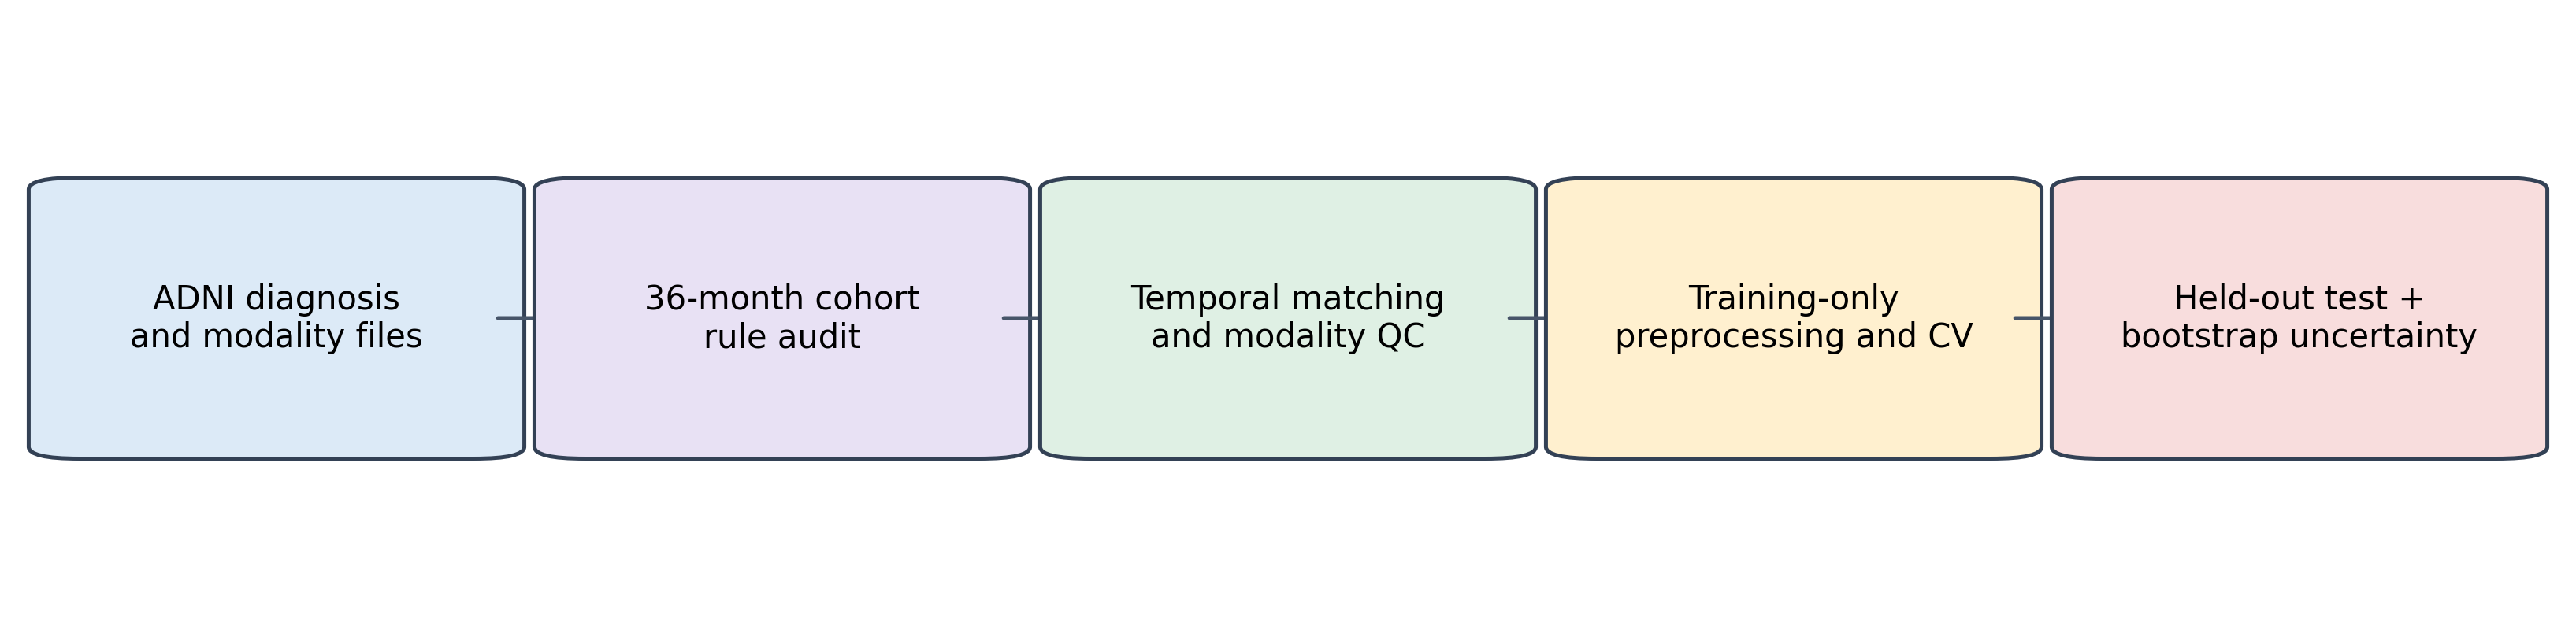
\includegraphics[width=\linewidth]{figures/reproducible_workflow.png}
    \caption{Reproducible ClinicalAlign-AD workflow. Access-controlled ADNI inputs are transformed into an auditable cohort and temporally matched modalities before participant-disjoint model development and held-out evaluation.}
    \label{fig:workflow}
\end{figure}

\subsection{Cohort Definition}
\label{subsec:cohort}

Longitudinal diagnoses were obtained from the ADNI diagnosis summary table. Current diagnosis was taken from the harmonized diagnosis field when available, supplemented by diagnostic-change and legacy current-diagnosis fields. Records with missing dates, dates before January 1, 2000, or dates after the data cutoff of September 20, 2026 were excluded.

Baseline was defined as the earliest visit coded as baseline with a current diagnosis of MCI. A participant was labeled as a converter if an AD diagnosis occurred within 1,095 days after baseline. A participant was labeled stable if no qualifying conversion occurred and a non-AD diagnosis was observed at or after day 1,005. This candidate rule produced 702 participants: 255 converters and 447 stable participants. A stricter definition requiring MCI, rather than any non-AD diagnosis, at qualifying follow-up produced 664 participants (255 converters and 409 stable participants). The candidate rule was retained because it reproduced the previously reported converter count and preserved participants whose later diagnosis was cognitively normal; however, it yielded seven more stable participants than the legacy count of 440. No participants were manually removed to force agreement.

A fixed stratified holdout assigned 561 participants to training and 141 to testing. The test set contained 51 converters and 90 stable participants. Participant identifiers did not overlap between splits.

\subsection{Data Sources and Temporal Matching}
\label{subsec:data_preparation}

Demographic and family-history variables were obtained from ADNI subject-characteristic tables. Baseline age, sex, education, and family history of dementia or AD formed the clinical core. Extended clinical features included body mass index, blood pressure, pulse, neurological-examination abnormality count, medical-history condition count, and selected history indicators.

Plasma NfL measurements were obtained from the longitudinal Blennow laboratory table; plasma NfL has previously shown associations with neurodegeneration and disease progression in AD cohorts \cite{mattssonAssociationPlasmaNeurofilament2017,lewczukPlasmaNeurofilamentLight2018}. DTI data included complete legacy version-1 scans and robust-mean version-2/3 regional summaries. Fractional anisotropy (FA), mean diffusivity (MD), axial diffusivity (AD), and radial diffusivity (RD) were summarized across available white-matter regions using row-level means and standard deviations, consistent with the use of regional DTI measures to characterize MCI and AD \cite{mielkeRegionallySpecificDiffusion2009,douaudDTIMeasuresMild2011,nirEffectivenessRegionalDTI2013}. Standard-mean version-2/3 DTI summaries were retained separately as a sensitivity representation.

FreeSurfer 7 outputs included hippocampal and amygdala volumes, lateral-ventricle volume, intracranial volume, total gray-matter volume, and temporal cortical thickness measures \cite{fischlFreeSurfer2012}. Records with an overall QC rating of Fail were excluded. Regional QC failures masked the affected features, and records labeled Hippocampus Only retained only hippocampal measures. Because the selected candidate cohort was primarily represented by FreeSurfer 7.2 records with partial processing status and without explicit overall QC scores, these structural-MRI analyses were designated exploratory.

Clinical measurements were eligible from 180 days before to 90 days after baseline. NfL, DTI, and FreeSurfer measurements were eligible from 365 days before to 90 days after baseline. The closest eligible record was selected, with pre-baseline measurements preferred when observations were equidistant. Measurements on or after the participant's outcome date were excluded. DTI scans with severe artifacts, failed DICOM conversion, incomplete acquisition, poor field of view, or failed atlas registration were excluded; less severe QC annotations were retained as warnings.

\subsection{Feature Configurations}

The prespecified clinical/NfL/DTI analysis used the following configurations:

\begin{itemize}
    \item \textbf{Clinical core:} age, sex, education, and family history;
    \item \textbf{Clinical extended:} clinical core plus summary variables from vital signs, neurological examination, and medical history;
    \item \textbf{Clinical core or extended + NfL:} addition of log-transformed plasma NfL;
    \item \textbf{Clinical extended + DTI:} addition of robust-primary DTI means and standard deviations; and
    \item \textbf{Clinical extended + standard-mean DTI:} an alternative DTI-processing sensitivity analysis.
\end{itemize}

Two structural-MRI configurations were evaluated separately as exploratory analyses: clinical extended plus FreeSurfer features and an all-modality configuration combining clinical, NfL, primary DTI, and FreeSurfer variables.

\subsection{Preprocessing and Models}

All preprocessing was estimated using training data only to prevent information leakage \cite{varoquauxMachineLearningMedical2022}. Numeric features were median-imputed and standardized. A binary missingness indicator was added for every feature with missing training observations. Sex was represented using a binary indicator. Within each training fold, imputation and scaling parameters were refitted rather than inherited from the full training set. Because simple imputation does not eliminate bias when missingness assumptions are violated, complete-case results were retained as a complementary sensitivity analysis \cite{Janssen2010,austinMissingDataClinical2021}.

Three dependency-light classical models were evaluated: L2-regularized logistic regression, Gaussian naive Bayes, and k-nearest neighbors. Hyperparameters were selected by five-fold stratified cross-validation within the training set using AUC. Logistic-regression penalty values were selected from $\{0.001,0.01,0.1,1,10\}$; Gaussian naive Bayes variance-smoothing values were selected from $\{10^{-9},10^{-6},10^{-3},0.1\}$; and the number of neighbors was selected from $\{5,11,21,41\}$. The classification threshold was chosen by maximizing Youden's index on training out-of-fold predictions. The held-out test labels were not used for preprocessing, hyperparameter selection, or threshold selection.

L2-regularized logistic regression was prespecified for the main modality-ablation table to avoid selecting a different model after inspecting test-set performance. Gaussian naive Bayes and k-nearest-neighbor results were retained in the reproducibility outputs as secondary model comparisons.

\subsection{Evaluation and Statistical Analysis}

The primary metric was the area under the receiver operating characteristic curve (AUC). Balanced accuracy, sensitivity, specificity, F1-score, and Brier score were also calculated to avoid reducing performance assessment to discrimination alone \cite{steyerbergAssessingPerformancePrediction2010,vancalsterCalibrationAchillesHeel2019}. AUC and threshold-dependent uncertainty intervals were obtained from 1,000 class-stratified bootstrap samples of the fixed test predictions. Paired bootstrap samples were used to compare logistic-regression AUCs against the clinical-core reference.

The primary analysis retained the full candidate cohort using training-derived imputation and missingness indicators. Complete-case sensitivity analyses used the same fixed split after restriction to participants with all features in a configuration. Complete-case models were considered feasible only when both outcome classes contained at least five participants in the test subset and at least ten participants in training.

\subsection{Reproducibility and Data Governance}

Raw ADNI participant-level data and participant-level derived files were retained locally and excluded from version control. Public repository content includes cohort and modality configurations, analysis scripts, unit tests, cryptographic input hashes, and aggregate results without participant identifiers. All random operations used the declared seed 20260920.

\section{Results}
\label{sec:results}

\subsection{Cohort Characteristics and Modality Availability}

The candidate cohort included 702 participants, with 255 converters (36.3\%) and 447 stable participants. Mean baseline age was 72.2 years and mean education was 16.1 years. Table~\ref{tab:cohort_characteristics} summarizes cohort characteristics.

\begin{table*}[!ht]
\centering
\caption{Candidate-cohort characteristics and modality availability. Continuous variables are mean (SD); categorical variables are n (\%).}
\label{tab:cohort_characteristics}
\small
\setlength{\tabcolsep}{4pt}
\resizebox{\textwidth}{!}{%
\begin{tabular}{lrrrrrrrr}
\toprule
Group & N & Age, years & Female & Education, years & Family history & NfL available & DTI available & FreeSurfer available \\
\midrule
Overall & 702 & 72.2 (7.5) & 279 (39.7\%) & 16.1 (2.7) & 424 (60.5\%) & 336 (47.9\%) & 127 (18.1\%) & 698 (99.4\%) \\
Stable & 447 & 71.6 (7.6) & 177 (39.6\%) & 16.2 (2.7) & 280 (62.8\%) & 251 (56.2\%) & 89 (19.9\%) & 443 (99.1\%) \\
Converter & 255 & 73.3 (7.1) & 102 (40.0\%) & 15.9 (2.7) & 144 (56.5\%) & 85 (33.3\%) & 38 (14.9\%) & 255 (100.0\%) \\
\bottomrule
\end{tabular}
}
\end{table*}

Clinical information was nearly complete. NfL was available for 336 participants (47.9\%), primary DTI for 127 (18.1\%), and standard-mean version-2/3 DTI for 43 (6.1\%). Exploratory FreeSurfer features were available for 698 participants (99.4\%). NfL availability differed between stable participants (56.2\%) and converters (33.3\%), demonstrating that modality missingness was potentially informative rather than random. Figure~\ref{fig:coverage} shows availability by outcome group.

\begin{figure}[!ht]
    \centering
    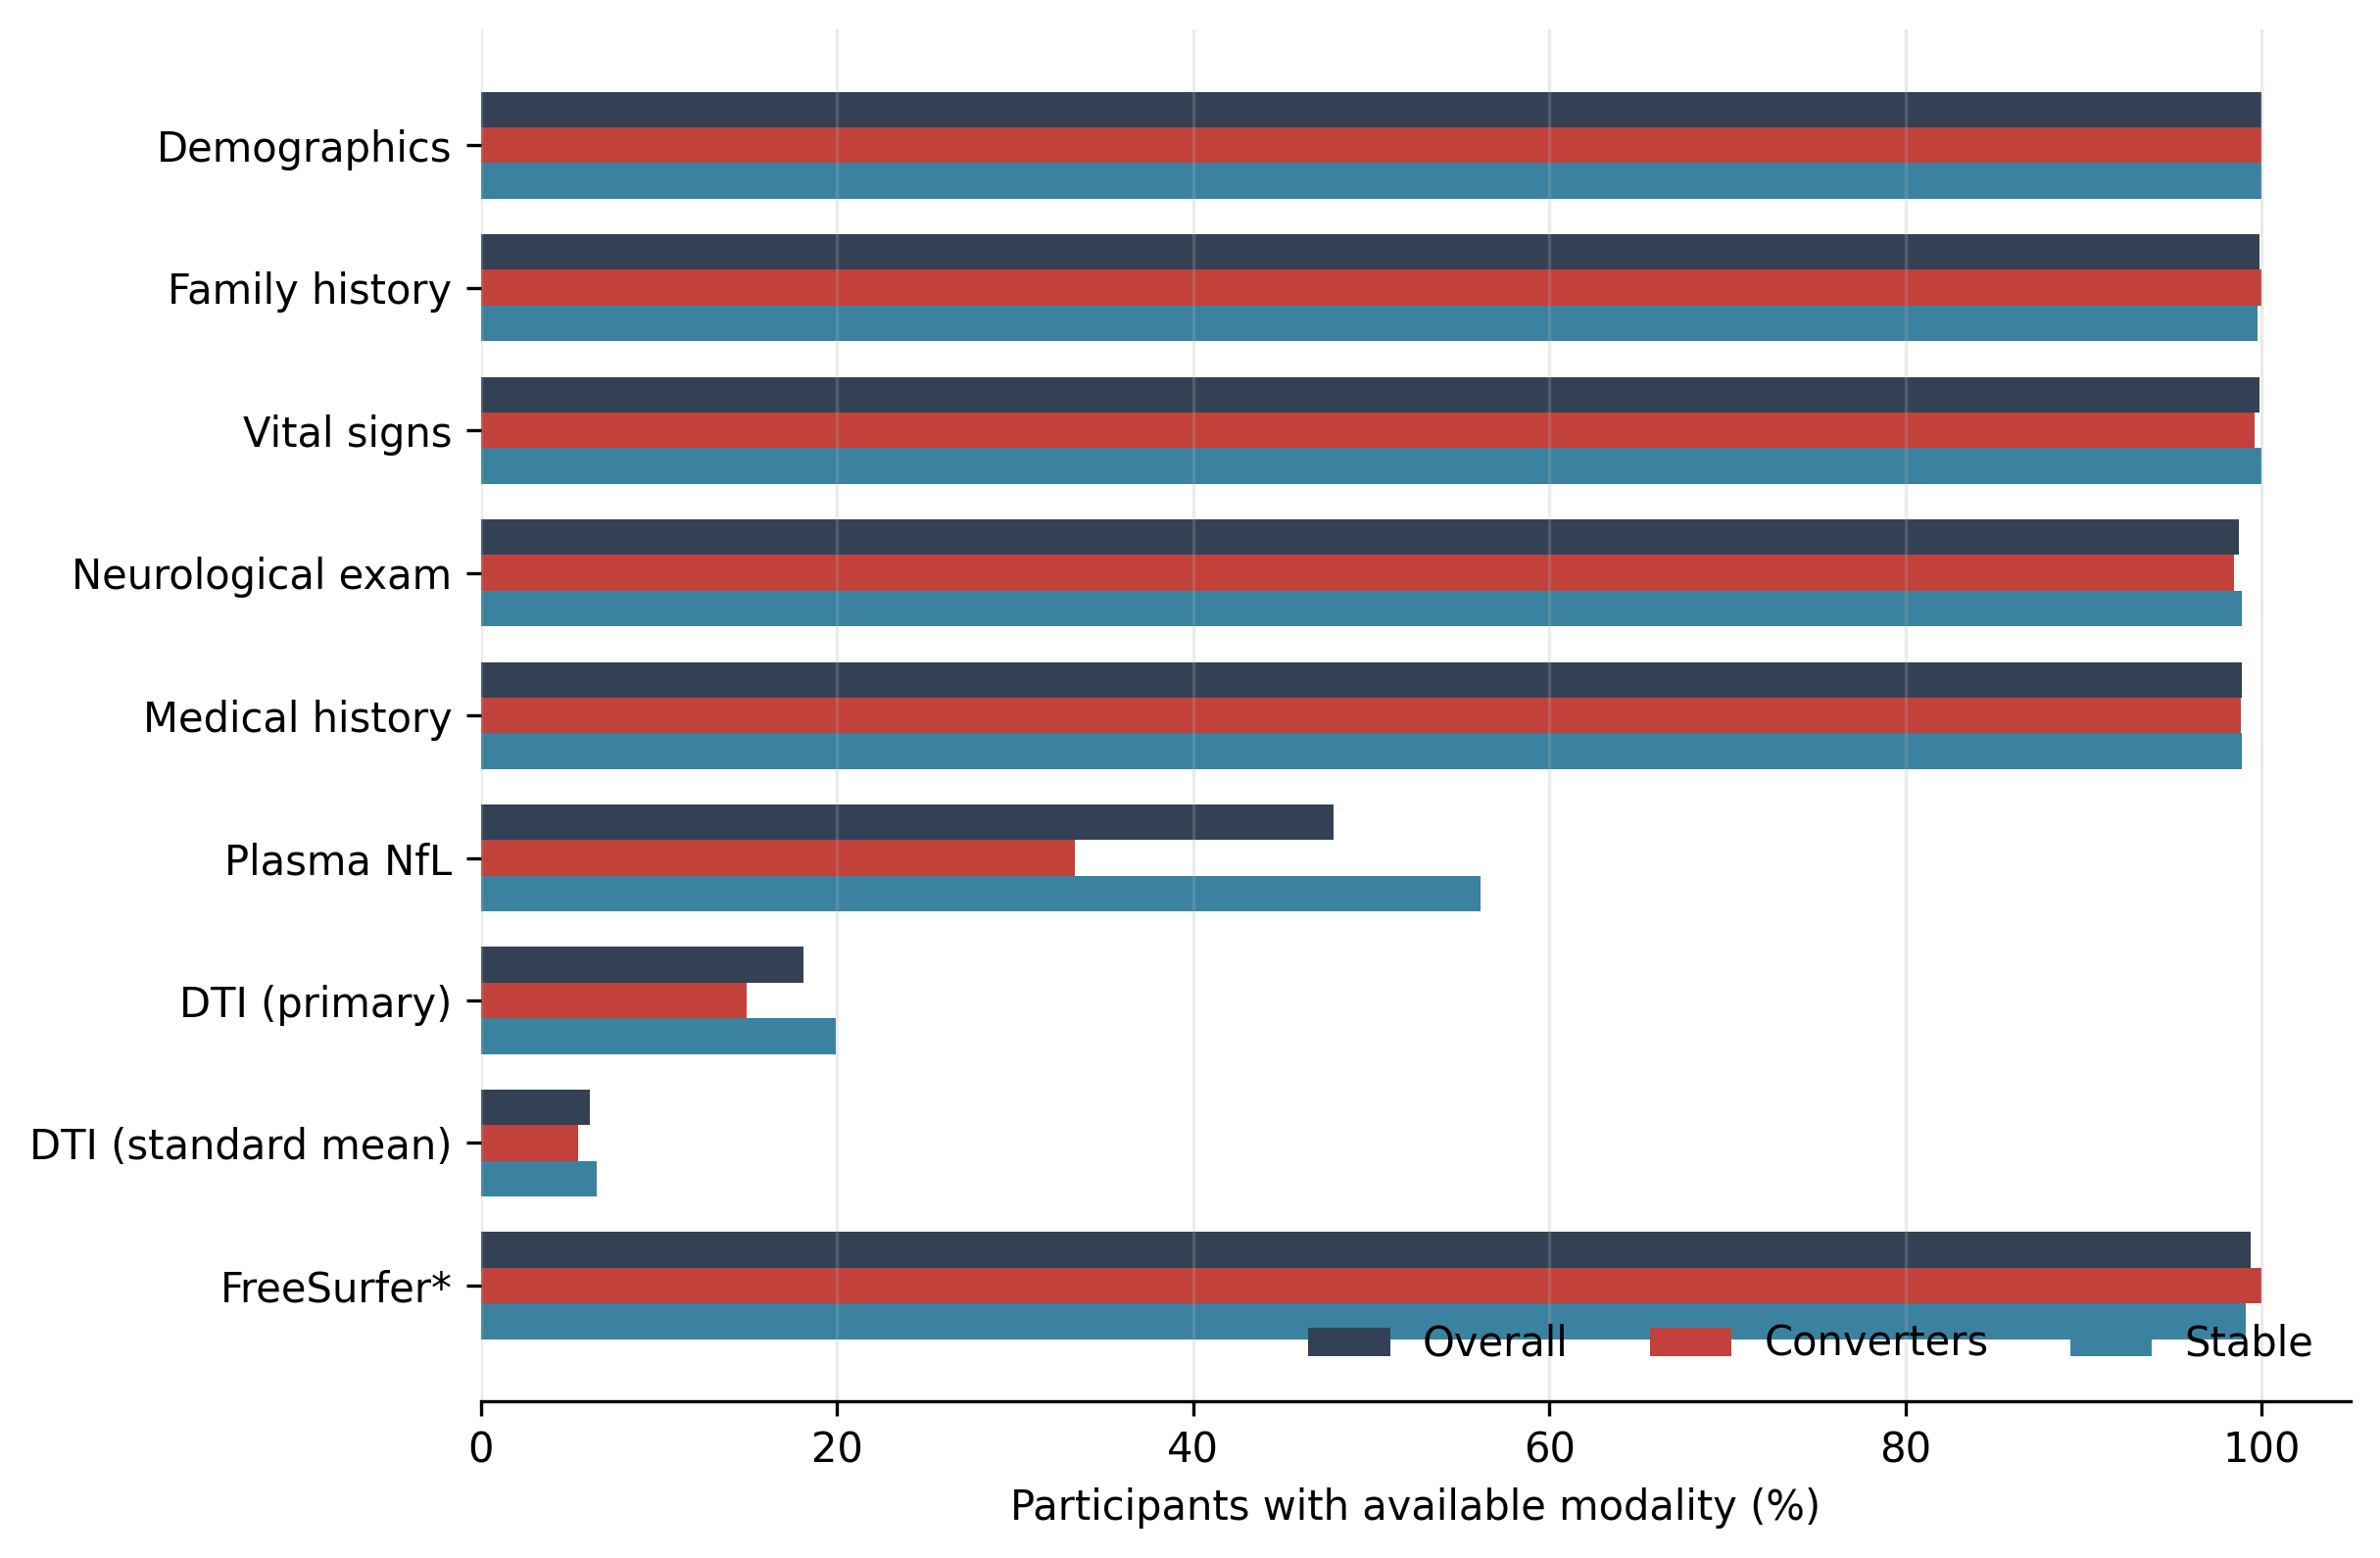
\includegraphics[width=0.92\linewidth]{figures/modality_coverage.png}
    \caption{Modality availability in the candidate cohort. FreeSurfer denotes an exploratory structural-MRI analysis.}
    \label{fig:coverage}
\end{figure}

\subsection{Held-Out Modality Ablations}

Table~\ref{tab:model_performance} reports the prespecified logistic-regression ablations on the same 141-participant held-out test set. Clinical core features achieved an AUC of 0.580 (95\% CI 0.486--0.674). Adding extended clinical variables increased AUC to 0.608 (0.515--0.699). Clinical core plus NfL achieved 0.640 (0.553--0.731), while clinical extended plus NfL achieved the strongest result within the prespecified clinical/NfL/DTI scope: 0.678 (0.590--0.762).

Primary robust-mean DTI features combined with extended clinical variables achieved an AUC of 0.636 (0.547--0.727). Standard-mean DTI produced a similar AUC of 0.628 (0.533--0.721). Relative to clinical core features, the paired logistic-regression AUC difference was 0.098 (95\% CI 0.001--0.193) for clinical extended plus NfL and 0.056 ($-0.022$--0.128) for clinical extended plus DTI.

\begin{table*}[!ht]
\centering
\caption{Held-out performance of the prespecified L2-regularized logistic-regression ablations. AUC confidence intervals use 1,000 class-stratified bootstrap samples.}
\label{tab:model_performance}
\small
\setlength{\tabcolsep}{5pt}
\resizebox{\textwidth}{!}{%
\begin{tabular}{lrrrrrr}
\toprule
Feature configuration & Test n & AUC (95\% CI) & Balanced accuracy & Sensitivity & Specificity & Brier score \\
\midrule
Clinical core & 141 & 0.580 (0.486--0.674) & 0.596 & 0.804 & 0.389 & 0.230 \\
Clinical extended & 141 & 0.608 (0.515--0.699) & 0.537 & 0.941 & 0.133 & 0.225 \\
Clinical core + NfL & 141 & 0.640 (0.553--0.731) & 0.649 & 0.843 & 0.456 & 0.213 \\
Clinical extended + NfL & 141 & 0.678 (0.590--0.762) & 0.636 & 0.706 & 0.567 & 0.210 \\
Clinical extended + DTI & 141 & 0.636 (0.547--0.727) & 0.593 & 0.765 & 0.422 & 0.221 \\
Clinical extended + standard-mean DTI & 141 & 0.628 (0.533--0.721) & 0.596 & 0.804 & 0.389 & 0.222 \\
Clinical extended + FreeSurfer* & 141 & 0.780 (0.703--0.848) & 0.678 & 0.667 & 0.689 & 0.178 \\
All modalities* & 141 & 0.802 (0.730--0.872) & 0.689 & 0.588 & 0.789 & 0.176 \\
\bottomrule
\end{tabular}
}
\begin{minipage}{0.98\linewidth}\footnotesize
*Exploratory structural-MRI analyses were not part of the original clinical/NfL/DTI analysis scope. Classification thresholds were selected from training-only out-of-fold predictions.
\end{minipage}
\end{table*}

The exploratory structural-MRI configuration achieved an AUC of 0.780 (0.703--0.848), and the exploratory all-modality configuration achieved 0.802 (0.730--0.872). Relative to clinical core features, the all-modality AUC difference was 0.222 (0.098--0.332). These structural-MRI results were stronger than the prespecified clinical/NfL/DTI analyses but should not be interpreted as confirmed superiority because they were exploratory and were not evaluated in an external cohort.

Figure~\ref{fig:auc_ablation} visualizes the held-out logistic-regression AUCs and bootstrap intervals.

\begin{figure}[!ht]
    \centering
    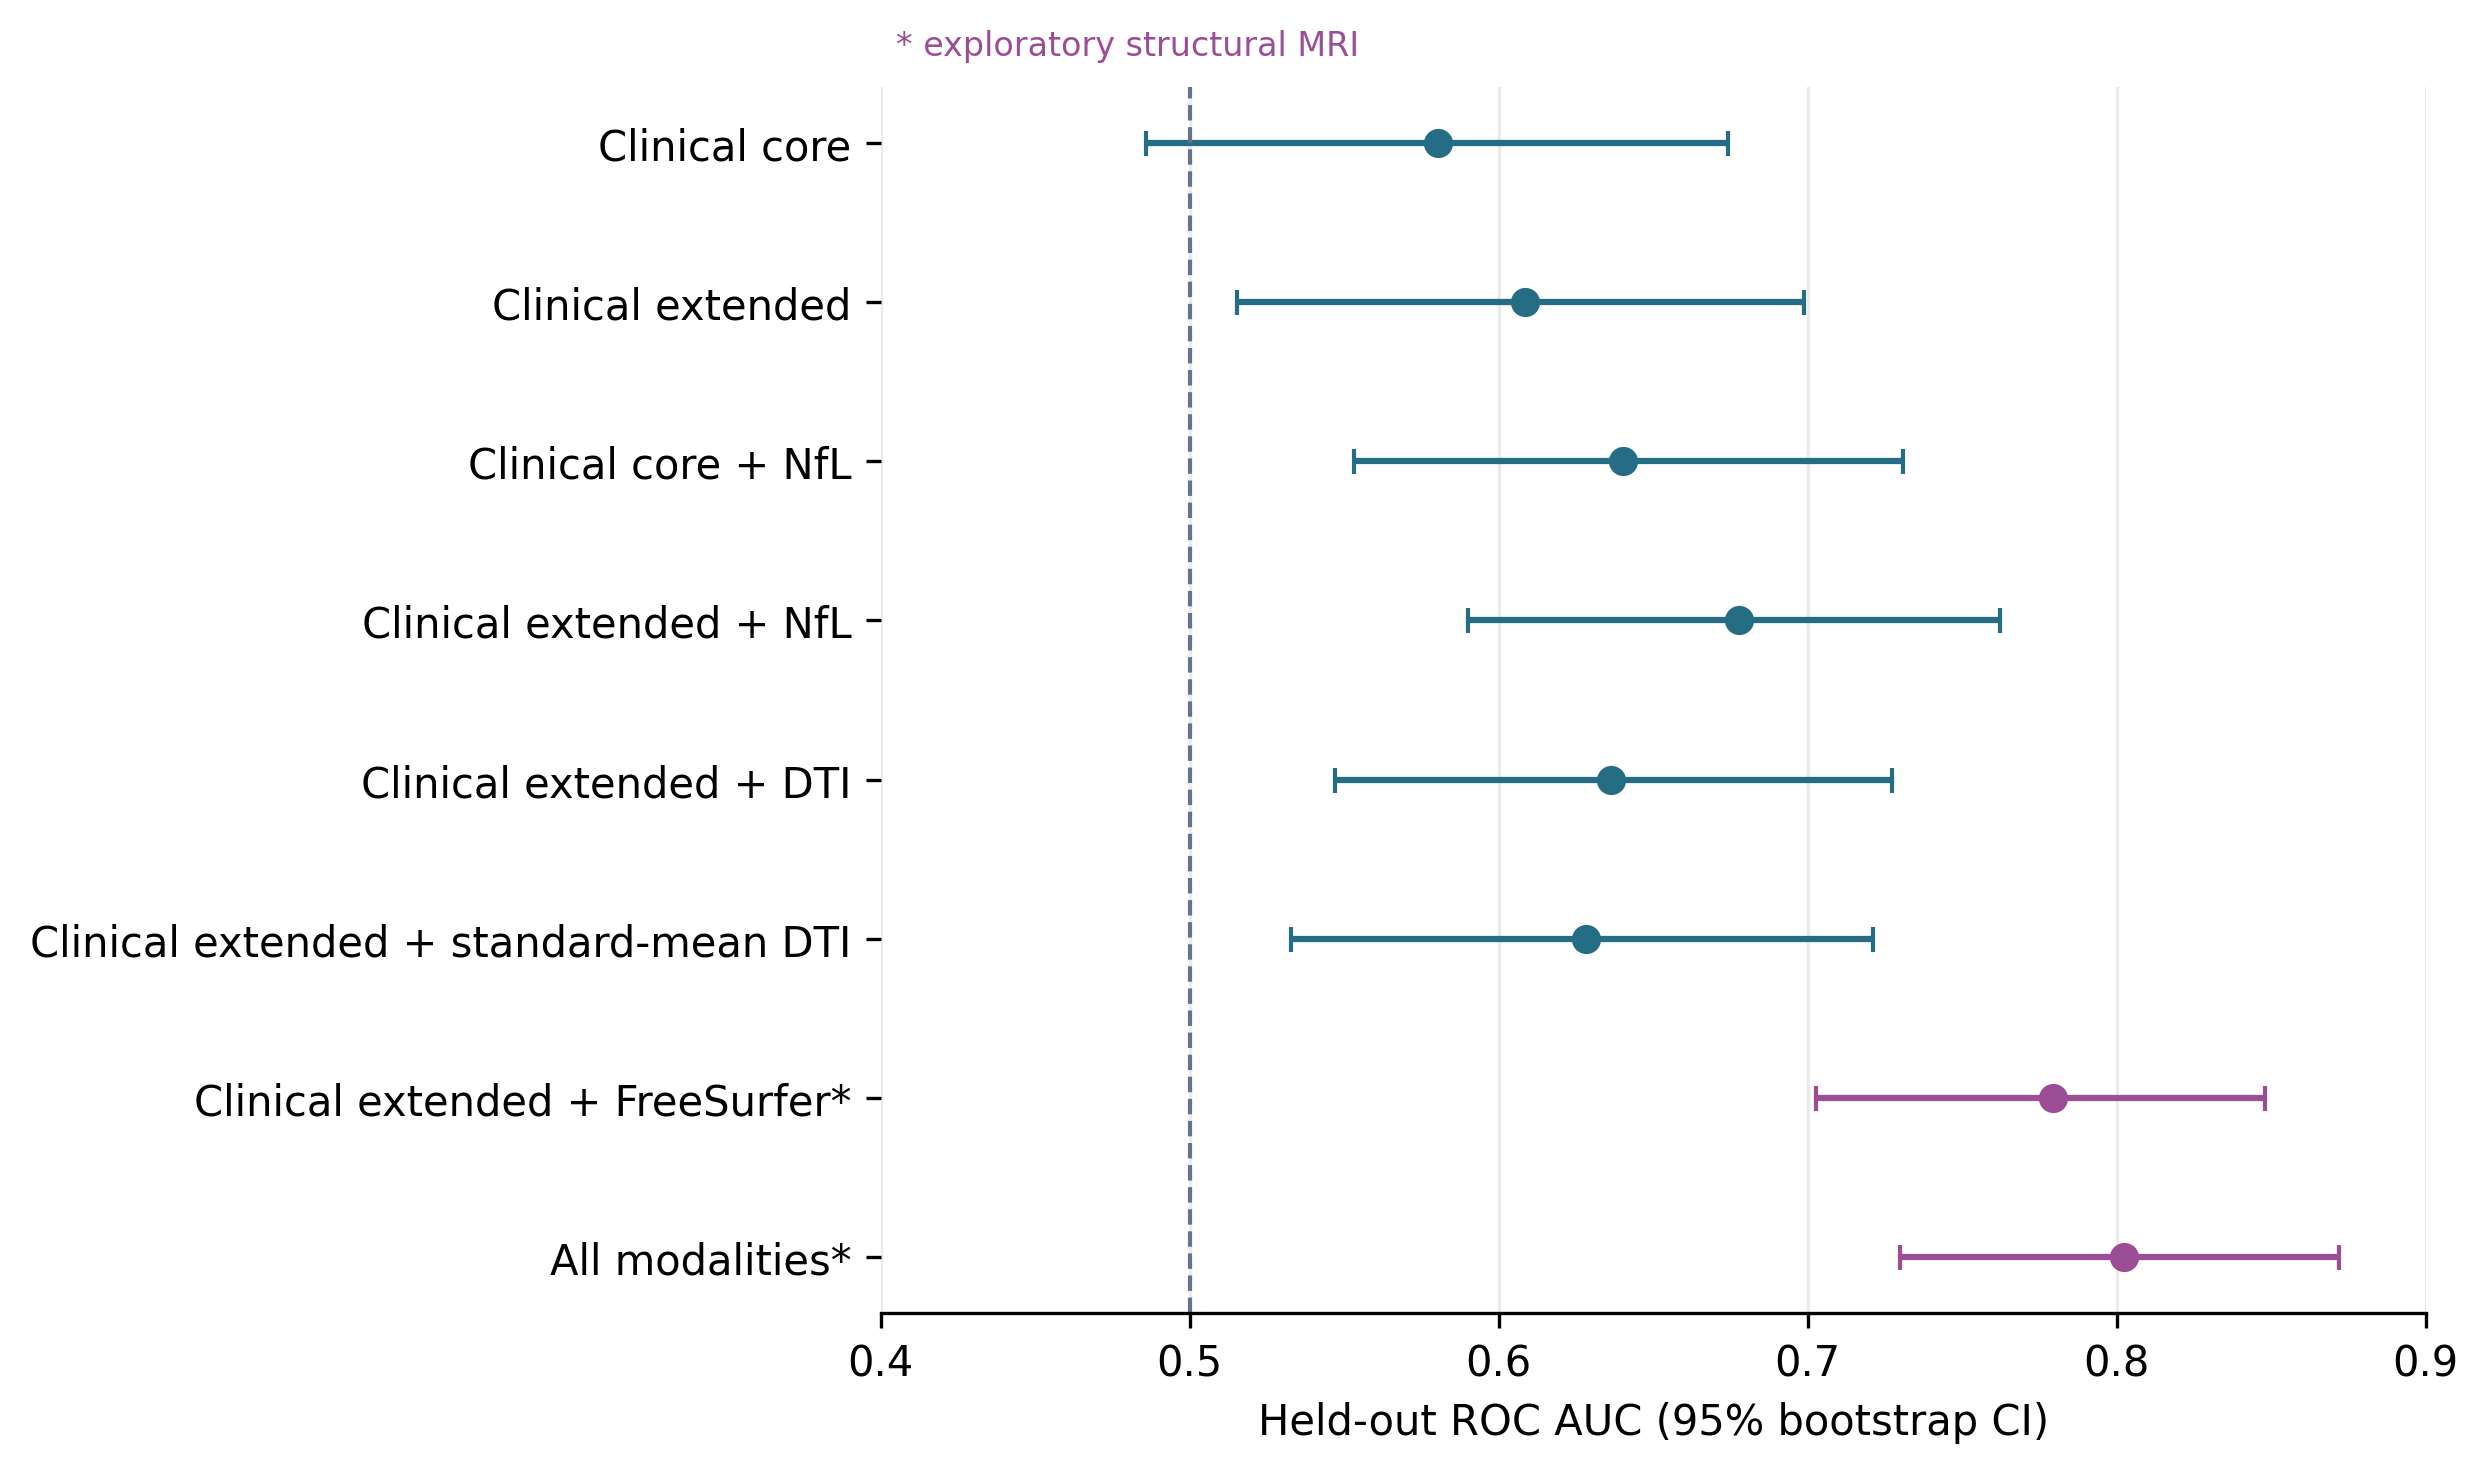
\includegraphics[width=0.92\linewidth]{figures/heldout_auc_ablation.png}
    \caption{Held-out ROC AUC for prespecified logistic-regression feature ablations. Purple entries denote exploratory structural-MRI analyses.}
    \label{fig:auc_ablation}
\end{figure}

Secondary model comparisons showed that no single algorithm dominated every configuration. Gaussian naive Bayes achieved an AUC of 0.668 for clinical extended plus primary DTI and 0.793 for clinical extended plus FreeSurfer, whereas logistic regression achieved the highest all-modality AUC of 0.802. Full secondary-model results and training-fold tuning records are provided in the aggregate reproducibility outputs.

\subsection{Complete-Case Sensitivity Analyses}

Complete-case analyses substantially reduced sample size. Clinical extended plus NfL retained 263 training and 66 test participants and achieved a logistic-regression AUC of 0.734 (0.597--0.852). The corresponding confidence interval was wider than that of the imputed full-cohort analysis. FreeSurfer complete-case analysis retained 550 training and 135 test participants and achieved an AUC of 0.757 (0.674--0.834).

\begin{table}[!ht]
\centering
\caption{Complete-case sensitivity analyses using logistic regression.}
\label{tab:complete_case}
\small
\setlength{\tabcolsep}{4pt}
\resizebox{\linewidth}{!}{%
\begin{tabular}{lrrrr}
\toprule
Feature configuration & Train n & Test n & Test converters & AUC (95\% CI) \\
\midrule
Clinical core + NfL & 267 & 68 & 15 & 0.633 (0.462--0.794) \\
Clinical extended + NfL & 263 & 66 & 14 & 0.734 (0.597--0.852) \\
Clinical extended + FreeSurfer* & 550 & 135 & 50 & 0.757 (0.674--0.834) \\
\bottomrule
\end{tabular}
}
\begin{minipage}{0.95\linewidth}\footnotesize
Complete-case DTI analyses were not estimated because the robust-mean DTI test subset contained only 4 converters; the all-modality complete-case subset contained one converter.
\end{minipage}
\end{table}

Complete-case primary DTI analysis retained only 98 training and 26 test participants; the test subset included four converters. The standard-mean DTI complete-case test subset contained eight participants, including three converters. These analyses did not satisfy the prespecified class-count threshold and were not estimated. The complete all-modality test subset contained only one converter and was also considered infeasible.

\section{Discussion}
\label{sec:discussion}

This study developed and applied a reproducible workflow for 36-month MCI-to-AD conversion prediction using heterogeneous ADNI-derived information. The main finding within the prespecified clinical/NfL/DTI scope was a modest improvement after adding NfL to extended clinical variables. DTI provided a smaller and statistically uncertain improvement, and its sparse availability prevented a reliable complete-case evaluation.

The NfL result is directionally consistent with reports linking plasma or serum NfL to neurodegeneration and clinical progression \cite{mattssonAssociationPlasmaNeurofilament2017,lewczukPlasmaNeurofilamentLight2018,preischeSerumNeurofilamentDynamics2019}, but it should be interpreted together with the availability pattern. NfL was observed more frequently among stable participants than converters. Consequently, full-cohort models with missingness indicators could use both the measured biomarker and the process determining whether the biomarker was available. Complete-case analysis removed this availability signal but produced a smaller and more selected test cohort. The difference illustrates why both imputed and complete-case analyses are informative but answer different questions \cite{Little2019,austinMissingDataClinical2021}.

The exploratory structural-MRI results were substantially stronger. Hippocampal volume relative to intracranial volume, ventricular burden, gray-matter volume, and temporal cortical thickness plausibly capture neurodegenerative change beyond basic clinical characteristics, consistent with prior longitudinal and machine-learning studies \cite{jackPredictionADMRIBased1999,devanandHippocampalEntorhinalAtrophy2007,shannonl.risacherBaselineMRIPredictors2009,eskildsenPredictionAlzheimersDisease2013,moradiMachineLearningFramework2015}. However, the FreeSurfer analysis was not part of the original clinical/NfL/DTI scope, most selected records had partial processing status without explicit overall QC scores, and no independent cohort was available. These results therefore motivate a confirmatory analysis rather than a claim of clinical readiness.

The cohort audit also identified a reproducibility issue. The explicit candidate rule reproduced the legacy converter count of 255 but produced 447 stable participants rather than 440. A stricter stable-MCI rule produced only 409 stable participants. Because no documented rule uniquely identified seven participants for exclusion, the analysis retained all 702 rule-eligible participants instead of forcing the historical total. This decision changes the held-out sample from the previously reported 139 participants to 141 and underscores the importance of publishing executable cohort definitions.

The model results further demonstrate the uncertainty associated with a single held-out sample. Even with 141 test participants, clinical-core AUC confidence intervals included 0.5, and complete-case intervals were wide. Adequate external-validation sample size depends on outcome frequency and the precision required for discrimination and calibration estimates \cite{rileyMinimumSampleSizeExternal2021}. Threshold-dependent measures also varied because thresholds were selected on training out-of-fold predictions rather than optimized on the test set. AUC, balanced accuracy, calibration, and clinical utility should therefore be considered jointly \cite{steyerbergAssessingPerformancePrediction2010,vancalsterCalibrationAchillesHeel2019}.

\subsection{Clinical and Informatics Implications}

For clinical informatics, the results emphasize that the apparent value of an added modality depends on more than its biological relevance. Coverage, acquisition timing, study phase, QC, and missingness mechanisms can determine whether a modality improves prediction. Systems intended for deployment should define how unavailable measurements are handled and should be evaluated under the same acquisition constraints expected in practice. Transparent reporting and formal risk-of-bias assessment can make these design choices visible to readers and external validators \cite{collinsTransparentReportingMultivariable2015,wolffPROBASTToolAssess2019}.

The reproducibility structure used here separates participant-level ADNI data from public code and aggregate outputs. This allows investigators with authorized ADNI access to reconstruct the analysis without redistributing restricted data. Explicit temporal windows and QC exclusions also make it possible to evaluate alternative assumptions without silently changing the cohort.

\subsection{Limitations}

Several limitations should be considered. First, this was a retrospective secondary analysis of ADNI rather than an external clinical validation. Second, the primary candidate cohort differed by seven stable participants from the legacy manuscript count; although this discrepancy was documented, its original cause could not be reconstructed. Third, post-baseline measurements up to 90 days were permitted to accommodate asynchronous baseline acquisition, although observations on or after the outcome date were excluded. A stricter pre-baseline-only sensitivity analysis should be considered in future work.

Fourth, NfL and particularly DTI were incompletely observed. Complete-case DTI evaluation was underpowered, while imputed models could exploit informative missingness; neither approach guarantees unbiased inference when the missingness mechanism is not adequately modeled \cite{Little2019,Janssen2010,austinMissingDataClinical2021}. Fifth, FreeSurfer findings were exploratory and require uniform regional QC and independent replication. Sixth, the dependency-light models evaluated here do not exhaust modern machine-learning or representation-learning methods. Their purpose was to provide transparent, reproducible baselines rather than establish a definitive optimal algorithm.

Future work should evaluate the workflow on independent longitudinal cohorts, prespecify external validation before structural-MRI model selection, investigate missing-not-at-random mechanisms, and compare pre-baseline-only with symmetric acquisition windows. Robust missing-modality models should be assessed only after adequate numbers of converters are available for each modality and with sufficient precision for both discrimination and calibration \cite{rileyMinimumSampleSizeExternal2021}.

\section{Conclusion}

ClinicalAlign-AD provides a transparent evaluation of clinical, NfL, DTI, and exploratory structural-MRI features for MCI-to-AD conversion prediction. NfL modestly improved discrimination beyond clinical characteristics, whereas sparse DTI availability limited reliable complete-case inference. Exploratory FreeSurfer features produced stronger held-out discrimination but require confirmatory validation. The study demonstrates that reproducible cohort rules, temporal alignment, modality QC, training-only preprocessing, and explicit uncertainty are central to trustworthy multimodal clinical prediction.

\section*{Ethics Statement}

This study used de-identified data obtained from the Alzheimer's Disease Neuroimaging Initiative (ADNI) database. The original ADNI study was approved by the institutional review boards of all participating centers, and written informed consent was obtained from all participants or their legally authorized representatives. The present work represents a secondary analysis of access-controlled de-identified data conducted in accordance with the ADNI Data Use Agreement.

\section*{Data Availability}

The data used in this study were obtained from the Alzheimer's Disease Neuroimaging Initiative database. Access is available to qualified investigators following approval and acceptance of the ADNI Data Use Agreement. Participant-level raw and derived data are not redistributed. Analysis code, configuration files, unit tests, input checksums, and non-identifying aggregate outputs accompany the manuscript repository.

\section*{Acknowledgments}

Data collection and sharing for this project was funded by the Alzheimer's Disease Neuroimaging Initiative (ADNI) (National Institutes of Health Grant U01 AG024904) and DOD ADNI (Department of Defense award number W81XWH-12-2-0012). ADNI is funded by the National Institute on Aging, the National Institute of Biomedical Imaging and Bioengineering, and through contributions from public and private partners. The investigators within ADNI contributed to the design and implementation of ADNI and/or provided data but did not participate in the analysis or writing of this report. A complete listing of ADNI investigators is available at:
\url{https://adni.loni.usc.edu/wp-content/uploads/how_to_apply/ADNI_Acknowledgement_List.pdf}

\bibliographystyle{elsarticle-num}
\bibliography{References}

\end{document}